Two point are P($x_{1},y_{1}$) and Q($x_{2},y_{2}$). The distance between both points is d.\\
\begin{align}
    \vec{Z} = \vec{P} - \vec{Q}  
\end{align}   
\vspace{0.5 cm}
Then the distance between P and Q is given by:

\begin{align}
   d = \norm{\vec{Z}}
\end{align}
\begin{align}
   d = \norm{\vec{P} - \vec{Q}} 
\end{align}

So, the distance between given points P and Q is:
\begin{align}
   d = \sqrt{(-2-3)^2 + (4-(-5))^2}    
\end{align}
\begin{align}
   d = \sqrt{25+81}    
\end{align}
\begin{align}
   d = \sqrt{106}    
\end{align}
So, the distance between P(-2,4) and Q(3,-5) is :
\begin{align}
   d = \sqrt{106}
\end{align}

\begin{figure}[t]
    \centering
    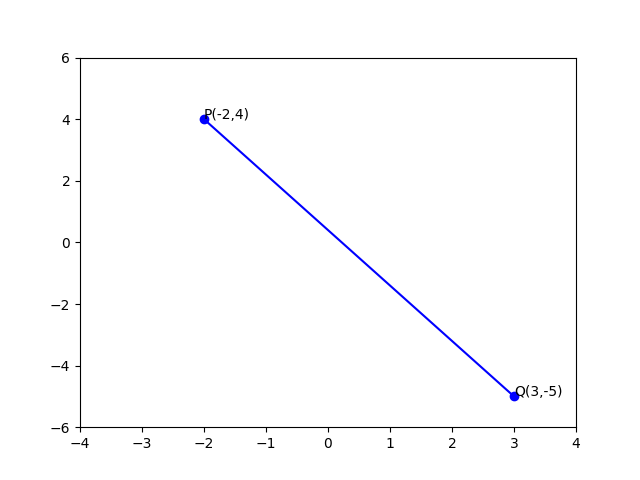
\includegraphics[width = \columnwidth]{./solutions/1/1/1/AI_assignment_1.png}
    \caption{Line between two points}
    \label{eq:solutions/1/1/1/fig:Line between two points}
\end{figure}


